\section{Introduction}

% Interest in building languages

All kinds of programmers are interested in building new languages. General-purpose languages evolve the slowest, but even so a dominant language like Java undergoes change over the years, adding new concepts and syntax\cite{java-generics}. Software engineers talk about how and when to build and use Domain Specific Languages\cite{fowler}. New compute architectures spawn new languages\cite{cuda}\cite{opencl}. Of course, programming language researchers are continually designing new languages to use or to analyze. Each new software innovation or fad brings with it a host of new markup languages. Yet the technology that is currently used to construct programming languages does not support these kinds of creative activities very well, and often the lack of good tool support is a major factor discouraging the creation and use of a new language.

The design and implementation of languages is often seen as a separate task from the creation of programs\cite{ward}\cite{intentional}. From another point of view the tasks of writing a program and building a language to write it in are naturally combined into one activity\cite{on-lisp}. These two perspectives go along with different tool sets, and the large disparity in goals and approaches suggests that there is room in the middle for \todo{...}

Furthermore, computer language technology could potentially be used in many more contexts as well. For instance, any class of structured documents (say recipes, essays, math problems) could be represented with a language defining the required elements and their relationships to each other. The tools used to create these documents are often far more user-friendly and visually rich than programming tools, but they fail to identify the underlying structure of the documents, trapping the data in a panorama of closed formats which obscure the valuable content. If the tools programmers use to create and work with languages offered better expressivity and were simpler to employ, software for creating many kind of documents could be built on similar foundations. 


% Approaches:

Figure \ref{fig-1}(a) illustrates the basic situation. A programmer has an idea for a program she wants her computer to run. To accomplish that, she needs to turn the image in her mind into an Abstract Syntax Tree (AST) which her computer can interpret or compile. But how is she going to construct this AST?

\begin{figure}[h]
  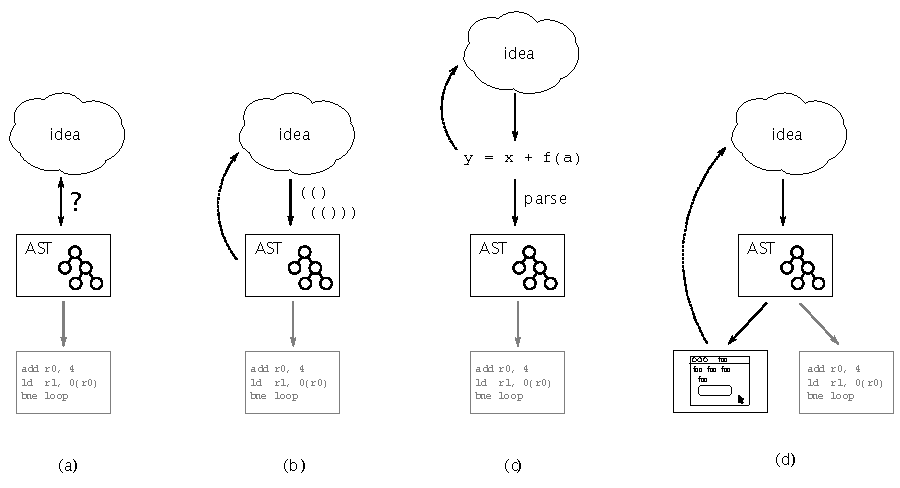
\includegraphics{src/image/figure1.pdf}
  \caption{\label{fig-1}The problem of turning an idea into a program, and three different solutions. Dashed arrows show the path of feedback from the computer to the programmer.}
\end{figure}

Figure \ref{fig-1}(b) shows the simplest solution. The programmer describes the AST directly in a form that requires little or no interpretation. For example, she can write a Lisp program in s-expressions, using parentheses to explicitly indicate the nested structure of her program. In doing so, she actually engages in a process of action and feedback. She types a bit, perhaps attempts to run the program, reviews the program's source text (really only a thinly-veiled AST), and then elaborates on or revises the program. The programmer is able to directly inspect the AST, but has to do so by counting parentheses.

These languages are easy to extend, but the extra effort required to read them is off-putting to the overwhelming majority of programmers.

Instead, they use the model diagrammed in Figure \ref{fig-1}(c), where another representation stands between the programmer and the AST. Now she enters her program as free-form text, which is interpreted by a parser as directions for constructing the AST. This allows for a more ``natural''-appearing syntax, but it also inserts a level of indirection between the programmer and her program. The feedback loop of idea to program and back now goes from mind to \emph{text} and back, without ever involving the AST. In fact, the AST is now a mere by-product of the source text. Until she runs her compiler and inspects its error messages, she doesn't even know whether the program makes any sense (if then!)

Furthermore, the parser imposes both limits and costs. The textual syntax must be carefully designed to achieve reasonable parser behavior, and changes are difficult and often mutually incompatible. Therefore, these languages tend to provide a single fixed syntax and the cost to change it is very high---you may have to convince a standards body to incorporate your idea, and then wait for compiler vendors to implement it.

A third approach is \emph{structure editing}. In Figure \ref{fig-1}(d), the programmer operates directly on the AST, but now the \emph{presentation} of the program is mediated by an editor. The first advantage of this setup is that the program's source is represented in the form of an AST, is edited at the level of the AST, and is always presented back to the user in terms of meaningful AST nodes. It's no longer possible for the programmer to \emph{read} the program one way while the parser disagrees. Secondly, the visual representation of the program---as well as the programmer's method of interacting with it---are not constrained to lines of text. The editor is free to supply more sophisticated layout, rendering, and forms of interaction.

Yet this power comes at a high cost. To construct a structure editor for a complete language is an effort undertaken only by researchers with teams of eager under-graduates at their disposal. Worse still, structure editors are too specialized and too limiting to be embraced by real working programmers, who have accepted the weaknesses of the parser-driven approach and have grown dependent on a universe of text-based tools. Thus structure editors find use only in certain niches (end-user programming, ...)\cite{??}.


% Solution:

This thesis presents a way out of this cage, by showing that a structure editor need not be a prison. It introduces a unified framework for constructing languages, editors, and compilers based on two simple ideas: all source code and derived objects are represented as ASTs, and a simple, extensible, functional, meta-language provides the glue to hold it all together.

\begin{figure}[h]
  \todo{1(d) with reduction to trees}
%  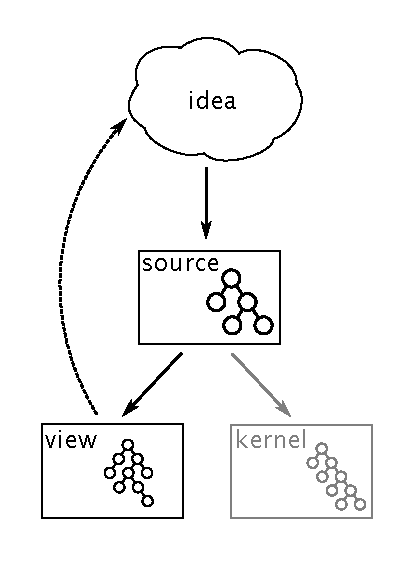
\includegraphics{src/image/figure2.pdf}
  \caption{\label{fig-2}\Meta}
\end{figure}

\temp{explain the diagram...}

\begin{enumerate}
\item When constructed this way, a structure editor can be flexible enough to work with whatever language you're using now or want to invent in the future.
\item Defining new language constructs or even entirely new languages can be made extremely simple, and the resulting language can be provided with the full services of the editing environment. Thus the barrier to entry for creating new languages is reduced to essentially zero.
\item Freed from the constraints of parsing, more sophisticated presentation becomes easy to achieve. The tools prototyped so far can achieve excellent readability for typical programming constructs, but also support rich, familiar, mathematical notation.
\end{enumerate}

I present a representation for ASTs and fundamental tools for manipulating them (Section \ref{ASTs}. Section \ref{languages} describes a way of defining languages. Section \ref{prototype} describes the prototyped system which implements these ideas, and section \ref{examples} presents examples of the system in use. 


